% vim: foldmethod=marker foldlevel=0

% -----------------------------------------------------------------------------
% information
% -----------------------------------------------------------------------------

\def \docAuthor {\question{Name:}\answer{Answer Key}}
\def \docClass  {CPSC 120}
\def \docSchool {~}
\def \docTerm   {Spring 2014}
\def \docTitle  {Worksheets}


% -----------------------------------------------------------------------------
% document setup
% -----------------------------------------------------------------------------
% {{{

\documentclass[12pt,letterpaper]{article}

\usepackage[includehead,
            includefoot,
            margin=1in,
            top=.25in,
            headheight=.75in,
            headsep=.25in,
            footskip=.25in,
           ]{geometry}

\usepackage[fleqn]{amsmath}
\usepackage{amssymb}
\usepackage{array}
\usepackage{enumitem}
\usepackage{fancybox}
\usepackage{fancyhdr}
\usepackage{l3regex}
\usepackage{mathtools}
\usepackage{minted}
\usepackage{multicol}
\usepackage{tikz}
\usepackage[normalem]{ulem}
\usepackage{url}
\usepackage{xcolor}


% text ------------------------------------------------------------------------

\binoppenalty = 10000  % never break next to a binary operator
\relpenalty   = 10000  % never break next to a relation operator

\setlength{\parindent}{0em}
\setlength{\parskip}{1ex}

\setlist[itemize]{nosep,itemsep=.5ex,parsep=.5ex}

% math ------------------------------------------------------------------------

\setlength{\mathindent}{1cm}

% - "\begin{document}" resets these values, so they have to be treated
%   specially
\AtBeginDocument{
  \setlength{\abovedisplayskip}{1.5ex plus .5ex minus .5ex}
  \setlength{\belowdisplayskip}{1.5ex plus .5ex minus .5ex}
}

% source code -----------------------------------------------------------------

\usemintedstyle{solarizedlight}

\fvset{samepage=true,frame=single,rulecolor=\color{.!30},framesep=2mm}

% header and footer -----------------------------------------------------------

\pagestyle{fancy}

\lhead{{\answer{\color{.}}\docClass}}
\rhead{{\answer{\color{.}}\docTitle}}
\cfoot{{\answer{\color{.}}\thepage}}
\renewcommand{\headrule}{{\answer{\color{red}}\hrule height 0.4pt}}
\renewcommand{\footrule}{{\answer{\color{red}}\hrule height 0.4pt}}

\fancypagestyle{firstpage}{
  \fancyhead[L]{{\answer{\color{red}}\docAuthor}
                {\answer{\color{.}}\\\docClass}}
  \fancyhead[C]{{\answer{\color{.}}\docSchool\\}}
  \fancyhead[R]{{\answer{\color{.}}\docTerm\\\docTitle}}
}


% -----------------------------------------------------------------------------
% macros
% -----------------------------------------------------------------------------

% abbreviations ---------------------------------------------------------------

\def \<{\langle}
\def \>{\rangle}

\def \ε{\varepisilon}
\def \θ{\vartheta}
\def \κ{\varkappa}
\def \π{\varpi}
\def \ρ{\varrho}
\def \σ{\varsigma}
\def \φ{\varphi}

\def \Γ{\varGamma}
\def \Δ{\varDelta}
\def \Θ{\varTheta}
\def \Λ{\varLambda}
\def \Ξ{\varXi}
\def \Π{\varPi}
\def \Σ{\varSigma}
\def \Υ{\varUpsilon}
\def \Φ{\varPhi}
\def \Ψ{\varPsi}
\def \Ω{\varOmega}

% special characters ----------------------------------------------------------

\catcode `α = \active \let α \alpha
\catcode `β = \active \let β \beta
\catcode `γ = \active \let γ \gamma
\catcode `δ = \active \let δ \delta
\catcode `ε = \active \let ε \epsilon
\catcode `ζ = \active \let ζ \zeta
\catcode `η = \active \let η \eta
\catcode `θ = \active \let θ \theta
\catcode `ι = \active \let ι \iota
\catcode `κ = \active \let κ \kappa
\catcode `λ = \active \let λ \lambda
\catcode `μ = \active \let μ \mu
\catcode `ν = \active \let ν \nu
\catcode `ξ = \active \let ξ \xi
\catcode `ο = \active \let ο o
\catcode `π = \active \let π \pi
\catcode `ρ = \active \let ρ \rho
\catcode `σ = \active \let σ \sigma
\catcode `τ = \active \let τ \tau
\catcode `υ = \active \let υ \upsilon
\catcode `φ = \active \let φ \phi
\catcode `χ = \active \let χ \chi
\catcode `ψ = \active \let ψ \psi
\catcode `ω = \active \let ω \omega

\catcode `Α = \active \let Α A
\catcode `Β = \active \let Β B
\catcode `Γ = \active \let Γ \Gamma
\catcode `Δ = \active \let Δ \Delta
\catcode `Ε = \active \let Ε E
\catcode `Ζ = \active \let Ζ Z
\catcode `Η = \active \let Η H
\catcode `Θ = \active \let Θ \Theta
\catcode `Ι = \active \let Ι I
\catcode `Κ = \active \let Κ K
\catcode `Λ = \active \let Λ \Lambda
\catcode `Μ = \active \let Μ M
\catcode `Ν = \active \let Ν N
\catcode `Ξ = \active \let Ξ \Xi
\catcode `Ο = \active \let Ο O
\catcode `Π = \active \let Π \Pi
\catcode `Ρ = \active \let Ρ P
\catcode `Σ = \active \let Σ \Sigma
\catcode `Τ = \active \let Τ T
\catcode `Υ = \active \let Υ \Upsilon
\catcode `Φ = \active \let Φ \Phi
\catcode `Χ = \active \let Χ X
\catcode `Ψ = \active \let Ψ \Psi
\catcode `Ω = \active \let Ω \Omega

% }}}
% other -----------------------------------------------------------------------
% {{{

% - sometimes a "\par", especially at the end of a block, is necessary to
%   prevent an extra (empty) paragraph from appearing in the output
% - `\color{.!50}` means 50 percent of the current color

\newlength{\currentparskip}

     \def \note     #1{{\color{.!50}#1\par}}
\long\def \longnote #1{{\color{.!50}#1\par}}

\def \ssQuestions {\filbreak\subsection*{Short Answer}}
\def \ssScope     {\filbreak\subsection*{Circle the Variables' Scopes}}
\def \ssMemory    {\filbreak\subsection*{Fill in the Memory}}
\def \ssFix       {\filbreak\subsection*{Fix the Broken Code}}
\def \ssTrace     {\filbreak\subsection*{Trace the Working Code}}

\long\def \textQuestion #1#2{%
  \filbreak
  \setlength{\currentparskip}{\parskip}
  \begin{minipage}[t][3.5in][t]{\textwidth}
    \setlength{\parskip}{\currentparskip}
    \subsubsection*{Question}
    #1
    \subsubsection*{Answer}
    \answer{#2}
  \end{minipage}
}

\def \codeScope #1{%
  \filbreak
  \vspace{1ex}
  \inputminted[frame=none,fontsize=\large]{c++}{./code/#1.cpp}
  \newpage
}

\def \codeMemory #1{%
  \filbreak
  \vspace{2ex}
  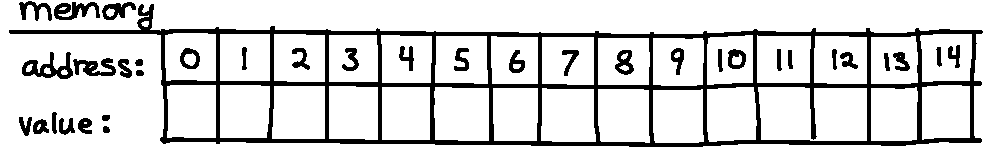
\includegraphics{./images/memory-0}
  \vspace{-2ex}
  \inputminted[frame=none,fontsize=\large]{c++}{./code/#1.cpp}
  \newpage
}

\def \codeFix #1{%
  \filbreak
  \question{
    \inputminted{c++}{./code/#1.cpp}
  } \answer{
    \inputminted{c++}{./code/#1.answer.cpp}
    \vspace{-6ex}
    \inputminted{diff}{./code/#1.answer.cpp.diff}
    \vspace{-6ex}
    \inputminted{text}{./code/#1.answer.cpp.output}
  }
  \vspace{-5ex}
}

\def \codeTrace #1{%
  \filbreak
  \inputminted{c++}{./code/#1.cpp}
  \question{
  } \answer{
    \vspace{-6ex}
    \inputminted{text}{./code/#1.cpp.output}
  }
  \vspace{-5ex}
}


% }}}
% -----------------------------------------------------------------------------
% document
% -----------------------------------------------------------------------------

\begin{document}
\thispagestyle{firstpage}

\newpage
\section*{Instructions}
For a each topic (if applicable) there are 5 sections:

\ssQuestions
Answer each question as well as you can.

\ssScope
Circle the scope of the given variables -- i.e., circle the part of the code in
which each variable ``exists''.  A good test, if you're not sure, is: if you
inserted a statement to \verb!cout! the variable at a given point in the code,
would any errors be produced?

\ssMemory
Fill in (or draw) a picture representing the computer memory, showing how the
variables might be allocated, and whether they have an assigned value, or are
uninitialized (use \verb!?! for ``uninitialized'').

\ssFix
Modify the code in the cleanest (and shortest) way possible, so that it will
compile and run without errors or warnings.

\ssTrace
Trace through the execution of the code, keeping track of the value of each
variable at each point in time, and the final output that the program produces.


\newpage
\section{Variables and Assignment}

\ssQuestions
\textQuestion{
  Describe undeclared variables, uninitialized variables, and initialized
  variables.
}{
  Undeclared variables don't really exist.  This term usually shows up in error
  messages when you try to use a variable that you haven't declared yet (either
  because you forgot, or you misspelled or mis-capitalized it, etc.).

  Uninitialized variables are declared, but have not yet been given a value.
  This means that their value is undefined (i.e., garbage, or whatever was in
  that location in memory before it was assigned to that variable).  Variables
  should not be used before being given a value.

  Initialized variables are both declared an initialized.  This means that they
  have been assigned a location in memory, and that that memory has been set to
  some desired value.
}
\textQuestion{
  Describe what we mean when we refer to a variable's scope.
}{
  A variable's scope is the region in the code where the variable ``exists''.
  Inside this scope, after the variable is declared, the variable may be used.
  Outside this scope, or before the variable has been declared, attempting to
  use the variable will result in a compile time error (in C++).

  In practice, the scope of most variables is determined by the innermost pair
  of curly braces containing it.

  It is possible for a variable in an inner scope to have the same name as a
  variable in an outer scope.  If this is the case, the variable in the inner
  scope is said to ``mask'' the variable from the outer scope, beginning from
  the point at which it is declared.  Once execution proceeds outside the inner
  scope, the variable from the outer scope will be ``visible'' (i.e., usable)
  again.
}
\newpage

\ssScope
\codeScope{1-scope-1}
\newpage

\ssMemory
\codeMemory{1-memory-1}

\ssFix
\codeFix{1-fix-1}
\codeFix{1-fix-2}
\newpage

\ssTrace
\codeTrace{1-trace-1}
\codeTrace{1-trace-2}
\codeTrace{1-trace-3}
\codeTrace{1-trace-4}
\newpage


\newpage
\section{Data Types and Expressions}
% TODO

\ssFix
\ssTrace


\newpage
\section{If and If-Else}
% TODO
% - *all* the different forms they can take

\ssScope
\ssMemory
\ssFix
\ssTrace


\newpage
\section{Boolean Expressions}
% TODO:
% - evaluating by hand

\ssScope
\ssMemory
\ssFix
\ssTrace


\newpage
\section{Predefined Functions}
% TODO
% - header files
% - usage
% - rand()
% - pow()

\ssScope
\ssMemory
\ssFix
\ssTrace


\newpage
\section{Loops}
% TODO: for, while, do-while
% - tracing
% - correspondence between the different types

\ssScope
\ssMemory
\ssFix
\ssTrace


\newpage
\section{Arrays}
% TODO
% - declaring
%   - uninitialized
%   - initialized
% - initializing with loops
% - initializing with cin
% - accessing a single element
% - swapping elements

\ssScope
\ssMemory
\ssFix
\ssTrace


\newpage
\section{Selection Sort}
% TODO

\ssScope
\ssMemory
\ssFix
\ssTrace


\end{document}

